%%
%% This is file `sample-manuscript.tex',
%% generated with the docstrip utility.
%%
%% The original source files were:
%%
%% samples.dtx  (with options: `manuscript')
%% 
%% IMPORTANT NOTICE:
%% 
%% For the copyright see the source file.
%% 
%% Any modified versions of this file must be renamed
%% with new filenames distinct from sample-manuscript.tex.
%% 
%% For distribution of the original source see the terms
%% for copying and modification in the file samples.dtx.
%% 
%% This generated file may be distributed as long as the
%% original source files, as listed above, are part of the
%% same distribution. (The sources need not necessarily be
%% in the same archive or directory.)
%%
%% The first command in your LaTeX source must be the \documentclass command.
%%%% Small single column format, used for CIE, CSUR, DTRAP, JACM, JDIQ, JEA, JERIC, JETC, PACMCGIT, TAAS, TACCESS, TACO, TALG, TALLIP (formerly TALIP), TCPS, TDSCI, TEAC, TECS, TELO, THRI, TIIS, TIOT, TISSEC, TIST, TKDD, TMIS, TOCE, TOCHI, TOCL, TOCS, TOCT, TODAES, TODS, TOIS, TOIT, TOMACS, TOMM (formerly TOMCCAP), TOMPECS, TOMS, TOPC, TOPLAS, TOPS, TOS, TOSEM, TOSN, TQC, TRETS, TSAS, TSC, TSLP, TWEB.
% \documentclass[acmsmall]{acmart}

%%%% Large single column format, used for IMWUT, JOCCH, PACMPL, POMACS, TAP, PACMHCI
% \documentclass[acmlarge,screen]{acmart}

%%%% Large double column format, used for TOG
% \documentclass[acmtog, authorversion]{acmart}

%%%% Generic manuscript mode, required for submission
%%%% and peer review
\documentclass[manuscript,screen,review,12pt]{acmart}
\usepackage{setspace}
\renewcommand{\baselinestretch}{1.0}
%% Fonts used in the template cannot be substituted; margin 
%% adjustments are not allowed.
%%
%% \BibTeX command to typeset BibTeX logo in the docs
\AtBeginDocument{%
  \providecommand\BibTeX{{%
    \normalfont B\kern-0.5em{\scshape i\kern-0.25em b}\kern-0.8em\TeX}}}

%% Rights management information.  This information is sent to you
%% when you complete the rights form.  These commands have SAMPLE
%% values in them; it is your responsibility as an author to replace
%% the commands and values with those provided to you when you
%% complete the rights form.
\setcopyright{acmcopyright}
\copyrightyear{2021}
\acmYear{2021}
%\acmDOI{10.1145/1122445.1122456}

%% These commands are for a PROCEEDINGS abstract or paper.
%\acmConference[Woodstock '18]{Woodstock '18: ACM Symposium on Neural
%  Gaze Detection}{June 03--05, 2018}{Woodstock, NY}
%\acmBooktitle{Woodstock '18: ACM Symposium on Neural Gaze Detection,
%  June 03--05, 2018, Woodstock, NY}
%\acmPrice{15.00}
%\acmISBN{978-1-4503-XXXX-X/18/06}


%%
%% Submission ID.
%% Use this when submitting an article to a sponsored event. You'll
%% receive a unique submission ID from the organizers
%% of the event, and this ID should be used as the parameter to this command.
%%\acmSubmissionID{123-A56-BU3}

%%
%% The majority of ACM publications use numbered citations and
%% references.  The command \citestyle{authoryear} switches to the
%% "author year" style.
%%
%% If you are preparing content for an event
%% sponsored by ACM SIGGRAPH, you must use the "author year" style of
%% citations and references.
%% Uncommenting
%% the next command will enable that style.
%%\citestyle{acmauthoryear}

%%
%% end of the preamble, start of the body of the document source.
\begin{document}

%%
%% The "title" command has an optional parameter,
%% allowing the author to define a "short title" to be used in page headers.
\title{A Searching Engine on Subject Description Form}

%%
%% The "author" command and its associated commands are used to define
%% the authors and their affiliations.
%% Of note is the shared affiliation of the first two authors, and the
%% "authornote" and "authornotemark" commands
%% used to denote shared contribution to the research.
\author{Yunfei LIU}
\authornote{These authors contributed equally to this research.}
\email{yunfei.liu@connect.polyu.hk}
%\orcid{1234-5678-9012}
\author{Jiaming HAN}
\authornotemark[1]
\email{jiaming.han@connect.polyu.hk}


\author{Zhuchen WANG}
\authornotemark[1]
\email{zhuchen.wang@connect.polyu.hk}



\author{longling GENG}
\authornotemark[1]
\email{long-ling.geng@connect.polyu.hk}
\affiliation{%
 \institution{The Hong Kong Polytechnic University}
 \streetaddress{Hung Hom}
 \city{Kowloon}
 \state{Hong Kong}
 \country{China}}


%%
%% By default, the full list of authors will be used in the page
%% headers. Often, this list is too long, and will overlap
%% other information printed in the page headers. This command allows
%% the author to define a more concise list
%% of authors' names for this purpose.
\renewcommand{\shortauthors}{Yunfei et al.}
\newcommand{\tabincell}[2]{\begin{tabular}{@{}#1@{}}#2\end{tabular}}
%%
%% The abstract is a short summary of the work to be presented in the
%% article.


%%
%% The code below is generated by the tool at http://dl.acm.org/ccs.cfm.
%% Please copy and paste the code instead of the example below.
%%
\begin{CCSXML}
<ccs2012>
   <concept>
       <concept_id>10003752.10003809.10010031.10010033</concept_id>
       <concept_desc>Theory of computation~Sorting and searching</concept_desc>
       <concept_significance>300</concept_significance>
       </concept>
 </ccs2012>
\end{CCSXML}

\ccsdesc[300]{Theory of computation~Sorting and searching}
%%
%% Keywords. The author(s) should pick words that accurately describe
%% the work being presented. Separate the keywords with commas.
\keywords{algorithm, searching, data structure, educution}

%% A "teaser" image appears between the author and affiliation
%% information and the body of the document, and typically spans the
%% page.
\begin{teaserfigure}
  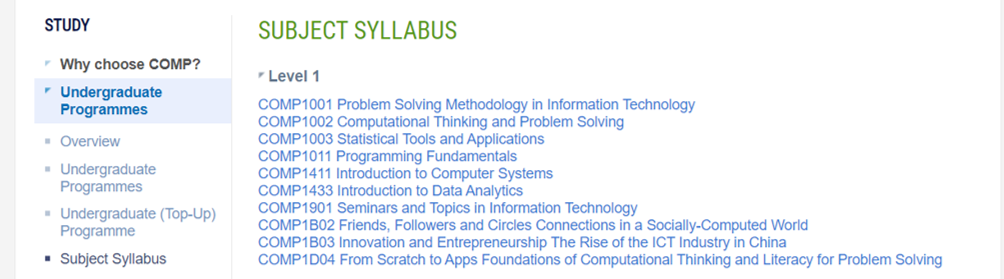
\includegraphics[width=\textwidth]{teaser}
  \caption{Subjects offered by PolyU COMP}
  \Description{Department of Computing in the Hong Kong Polytechnic University offers 81 undergraduate subjects}
  \label{fig:teaser}
\end{teaserfigure}

%%
%% This command processes the author and affiliation and title
%% information and builds the first part of the formatted document.
\maketitle

\section{Introduction}
Nowadays, many messages, webpages are created every day and we can't read them one by one. To get data quickly and effectively, searching is of vital importance. Meanwhile, how to search for the needed information in the shortest time, and how to find the correct webpages in numerous web pages on Internet, is a challenging question.

The searching algorithm is developed to save people's time of finding what they want, and it has a long history. Since the first search engine \textit{WebCrawler} appeared in 1994, humans have entered the information era. In this project, we revisited this part of history and figured out how the search engine is working. We developed our own data structures and algorithm to accelerate the searching process. Although our method is not mature enough, it is a good start for us to improve our programming skills and learn some experience.

\section{Algorithm}
We referenced the algorithm of \textit{ElasticSearch}, which is powerful, open-source, and easy to understand \cite{gormley2015elasticsearch}. However, even though the searching method is easy for experienced programmers, it is too complicated for us. Also, the data amount is small in this project, and complicating algorithms may lead to opposite effects \cite{divya2013elasticsearch,hogan2014fast}. Therefore, we learned the algorithm thoroughly and understand its essence. Finally, we simplified the algorithm, making it easier to program with just a slight increase in the searching time \cite{moschovakis2001algorithm}.

The main idea of this algorithm is to use a dictionary to search for the data. Firstly, users' input will be cleaned, which means that the special characters, numbers, punctuations will be removed, and uppercase letters will be transformed to lowercase letters. By doing these, users' input will be transformed into snippets that only contain lowercase alphabet, and it will be very helpful for further matching.

Then, the word snippets will be translated to word ID with a black-red tree dictionary \cite{li2004memory}. The black-red tree is an advanced self-balanced binary search tree, and the time complexity is $O(log n)$, which can shorten the searching time significantly. 

\section{Data Structure}

To implement the idea of object-oriented programming, as well as make the best use of C++ features, we defined two classes to represent subjects and words separately. 

The first class named \textbf{Course}, each instance represents one subject, contains essential information related to the subject including subject ID, subject code, subject pre-requisite, subject level, subject credit, and subject content. To implement the red-black tree, we use C++ STL container `map`, which is a balanced hash table \cite{das2008speeding}. It can search objects quickly. We use the map to store how many times the word appeared in this subject description form content. Meanwhile, in our opinion, the words that appeared in the title are much more important than the words that appeared in the content. Therefore, we assigned more impact index on words that appeared in the title, and use two map objects to store the title and content. Also, we think that data security is of vital importance in nowadays society, so we use private objects to store the data, which is safer and easier for future maintenance \cite{oualline2003practical,shaffer1997practical}. 

\begin{figure}[h]
  \centering
  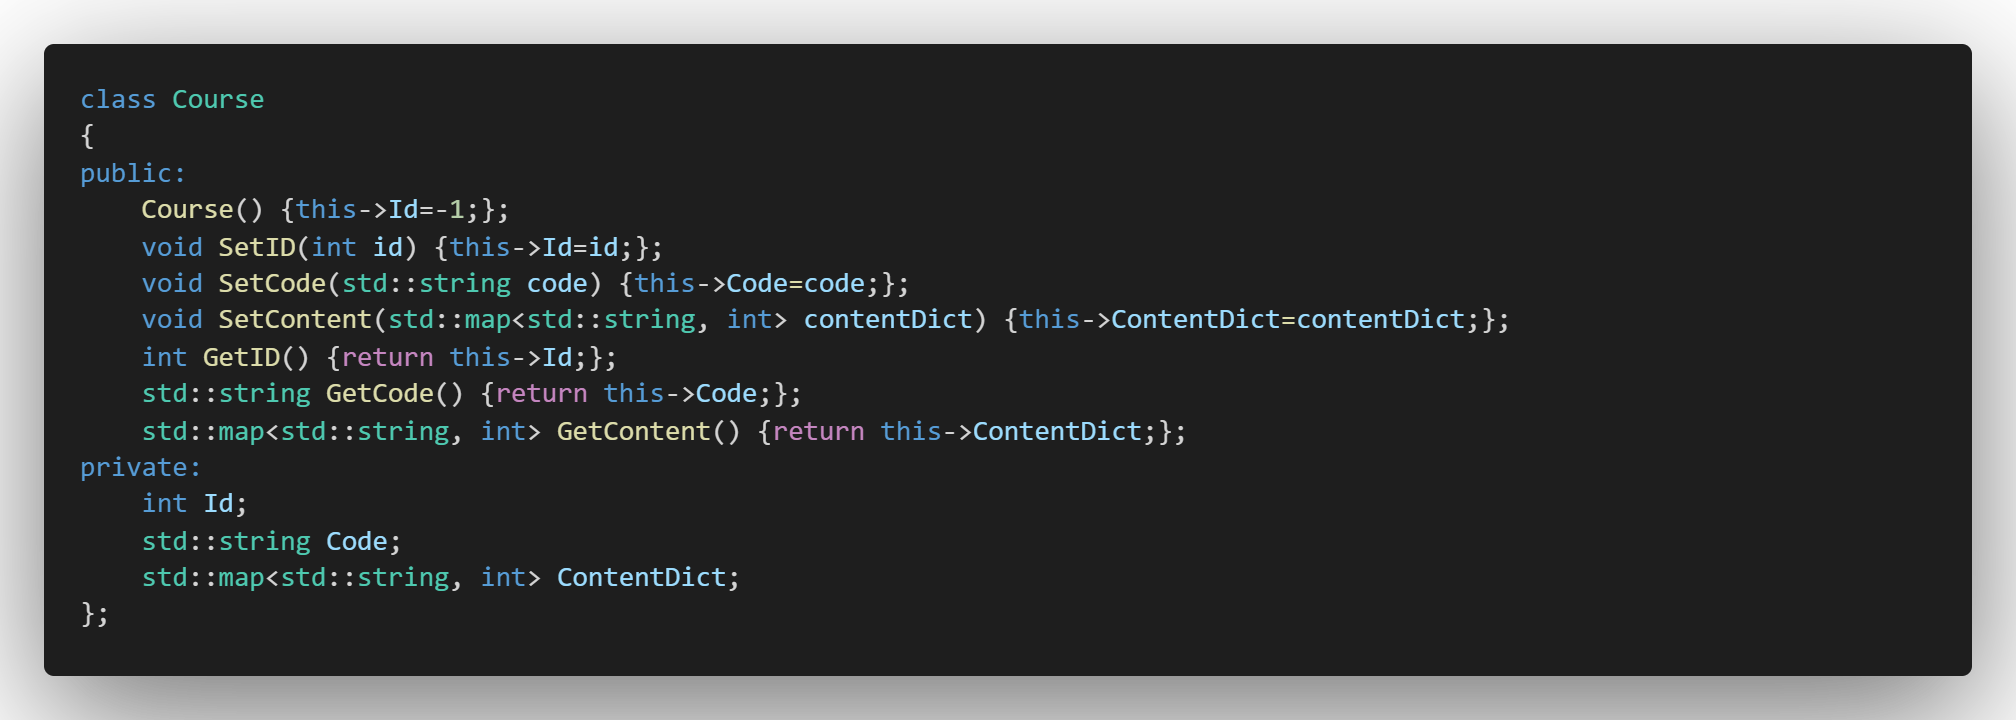
\includegraphics[width=\linewidth]{simplifiedcourse.png}
  \caption{A part of \textbf{Course} class, showing public and private objects}
  \Description{The C++ class}
\end{figure}

The second class names \textbf{Dictionary}, each instance represent one word that has appeared at least once in the subject description form contents. The class includes word name, word ID, the subject id where the word appeared in title or content. We use word ID to shorten the search time and make it easier to be searched in the whole content. Each Dictionary object contains one word, and the total amount of words is around 5000. Therefore, we defined an array of Dictionary objects to store all the words, and by accessing this array, the program can read all the information it needs. Also, we make good use of C++ STL containers, we choose to use a set to store the subject ID that the word has appeared, which can save time when searching \cite{prata2002c++}.

\begin{figure}[h]
  \centering
  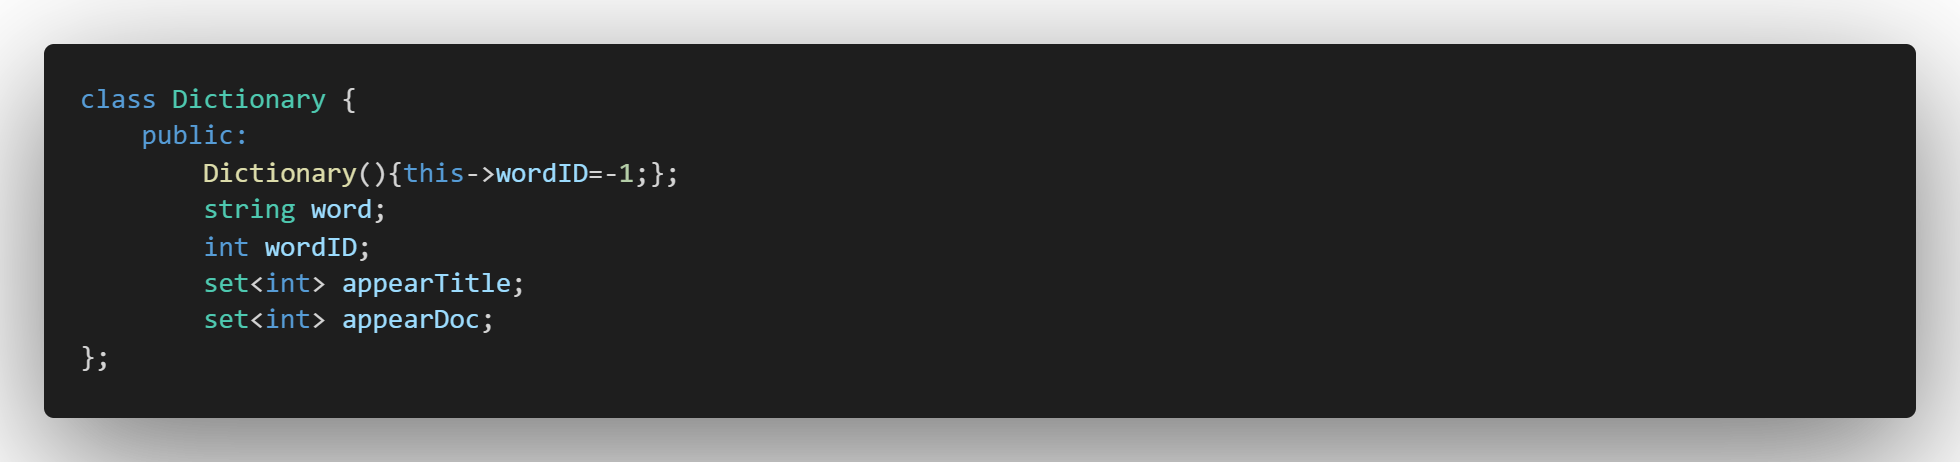
\includegraphics[width=\linewidth]{simplifieddictionary.png}
  \caption{The C++ code of \textbf{Dictionary} class}
  \Description{The C++ class}
\end{figure}

\section{Program Design}

\subsection{Overview}
For the data preparation part, we use \textit{Python} because of its flexibility and cross-platform feature. Since it is a C++ project, we only use Python downloading and transforming data, because C++ does not have libraries that can process \textit{PDF} files. Considering that the program may be implemented on the web later, and we want to leave some immigration ability to make it easier to run on different platforms, we use \textit{JSON} to save and process the data, which is a widely used data type between frontend and backend \cite{nurseitov2009comparison}. 

\subsection{Ideas}
To make the program easier to maintain, we try to use object-oriented programming skills. We divided the whole program into different functions, and each function can finish one small task, and they can be used as objects. By doing this, adding more functions becomes easy and convenient \cite{lafore1997object}.

\subsection{Problem-Solving}
We have divided the program into the follow four parts:

\begin{itemize}
    \item Data Pre-Process
    \item User Input Process
    \item Relative Index Calculation
    \item Result Display
\end{itemize}

To solve the problem of searching, we should first establish a database which stores all data. Then, we should check the users' input to avoid bugs caused by invalid input. After that, we should calculate the words relative index and finally display the searching result.

The relative index calculation formula is displayed as follows:

\begin{equation}
    R.I. = \sum_{i} \left[ N_{i(title)} \times 100 + N_{i(content)} \times 5 \right]
\end{equation}

While $N_{i(title)}$ represents the times that keywords shown in subject title and $N_{i(content)}$ represents the times that keywords shown in subject content.

\subsection{Designed Functions}
\begin{enumerate}
    \item \textbf{Input cleaning} \\
        Ask user to type the keywords, and then remove the unnecessary characters such as ",","'","@\&*", etc. Transform all uppercase letters to lowercase. \\ 
         \textit{\textbf{string* InputCleaning()}}: should return a pointer pointing to a string array, which needs to contain processed words user typed

    \item \textbf{Relevance Calculation} \\
        This function should integrate with the third function, and it should calculate the relevant score of each document. \\
        A algorithm which can represent the relevance of documents, you have this information: word input by users, how many times the word appear in the title of each document and how many times the word appear in the content of each document.

    \item \textbf{Dictionary Lookup} \\
        This function receives parameters including the return value of the previous function \textit{InputCleaning()} and dictionaries, and should search in the dictionary with the method of ElasticSearch. \\
        \textit{\textbf{int *Search(string *inputs)}}: should return a pointer pointing to an integer array. the array contains the scores of each subject description form

    \item \textbf{Result Display} \\
        After calculation, the search documents should be displayed in order, and the program should allow users interact with files, such as choose to display the content, or choose to download the pdf file.\\
        \textbf{\textit{void DisplayResult(float *scores)}}: display the search result and offer some interactions.
\end{enumerate}

\section{Data Process}
\subsection{Data Collection}
As required in the project description, the data we need is on the PolyU website \url{https://www.comp.polyu.edu.hk/en-us/study/undergraduate-programmes/subject}. The content of the website includes all course numbers, names, and description forms. To analyze them, we need to download them first then process them.

To download the files, the implementation of C++ of downloading files from a webpage is very complicated. Therefore, we use Python as an alternative method. Third-party libraries including \textit{urllib} and \textit{bs4} are used for processing the webpage and search for pdf files. The Python script is attached in the \textbf{DataCollectionPythonScript} folder \cite{richardson2007beautiful}.

\subsection{Data Transform}
Of course, C++ cannot process PDF files directly because they are not plain text. To get rid of this problem, we need to transform the PDF files to plain text. Python is used again because of its convenience. The third-party library \textit{pdfplumber} is used to transform the subject description forms to TXT files \cite{chen2016information}.

\subsection{Data Cleaning}
The subject description forms in TXT format are messy and cannot be used by C++ programs directly, so we need to clean the useless characters, and extract features from the TXT files. A Python script \textit{getfeature.py} attached in the \textbf{DataCollectionPythonScript} folder solves this problem. The script transforms the \textit{txt} files to \textit{JSON} format with the features including subject code, title, level, credit, pre-requisite, and content. The content is also transformed into JSON format to record each word and its appeared times. By cleaning data, the C++ program can process it faster and more conveniently \cite{lutz2001programming}.

\section{Discussion}
We have finish the required tasks successfully, and we add more functions to make the program more powerful, such as searching content and download the subject description forms. However, there are more things we can do. For example, we can move the program in a docker so that it can run everywhere. Also, we can program an webpage similar to Google for general public to use. Moreover, we can use SQL instead of JSON to allow larger data amount and frequently addition or deletion. The algorithm can be improved to adjust high concurrency, too.

\section{Challenges}
The first challenge we encountered is that the C++ do not have libraries which can process JSON files. Luckily, we finally found a third-party header which is called \textit{nlohmann json}. This library can process json files and transform it to C++ STL containers such as \textit{set} and \textit{map} \cite{skinner1992c++}.

The second challenge we encountered is class design. We should abstract the data and fit them with a framework. After several attempts, we finally create two classes for them.

The third challenge is the docking between different programmers. As the functions are written by different programmers, the arguments and return value expected are different. After communications, we reached the agreement.

\section{Conclusion}
In this program, we gain experiences about how to develop a program from the beginning to the end. We meet many problems and we have to find solution to it by ourselves. In this process, we learn a lot knowledge that we cannot learn in class. Also, during the presentation, we know how to show our achievements to public. All in all, developing this project is a valuable experience.

\newpage
\section{Appendix}
\subsection{Work Distribution}


\begin{center}
  \begin{tabular}{ccl}
    \toprule
    \textbf{Name} & \textbf{Work} \\
    \midrule
    \tabincell{c}{Yunfei LIU} & \tabincell{c}{Data Collection, Data Transform, Data Structure, Demo Make,\\Bug Fix, Program Combine, Report, Presentation Slides} \\ 
    \midrule
    Jiaming HAN& Algorithm Design, Relative Index Calculation\\
    \midrule
    Zhuchen WANG& Result Display, Demo Make\\
    \midrule
    Longling GENG& User Input Process, Demo Make \\
    \bottomrule
  \end{tabular}

\end{center}

\subsection{Useful links}
\begin{enumerate}
    \item GitHub Repository (Public on May 12) \url{https://github.com/liu-yunfei/COMP1011GroupProject}
    \item Subject Description Form Download Page \url{https://19040822.xyz/}

\end{enumerate}
\bibliographystyle{ACM-Reference-Format}
\bibliography{sample-base}


\end{document}
\endinput
%%
%% End of file `sample-authordraft.tex'.
